\chapter{Background \& Motivation}
\label{sec:background}

\begin{figure}[h]
\begin{center}
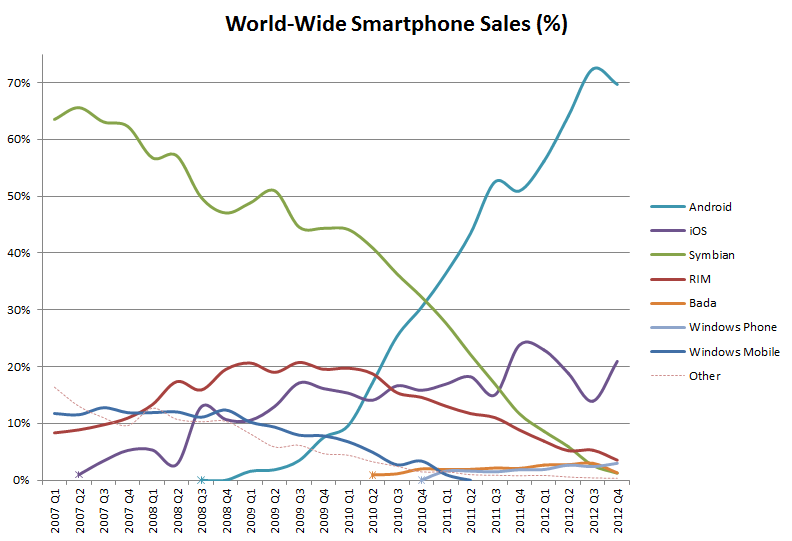
\includegraphics[width=0.8\columnwidth]{figs/World_Wide_Smartphone_Sales_Share}
\caption{Worldwide Market Share of various mobile OSs - from \citep{wikimobileshare} and \citep{gartnerq42012}}
\label{fig:mobileshares}
\end{center}
\end{figure}


Mobile OSs, like the PC operating systems of the 1990s, have a few major players that wield the most influence, as seen in Figure \ref{fig:mobileshares}. The two largest operating systems in the mobile area are Android and iOS. Apple's iOS, made exclusively for the Apple iPhone and iPad, as of the end of 2012, runs on over 20\%\citep{gartnerq42012} of all smartphones globally. Google's Android, released as an open source OS, has many different hardware manufacturers, Samsung, LG, HTC, Motorola, and many more. It currently runs the majority of smartphones globally, with 70\%\citep{gartnerq42012}  marketshare. Some of the less popular, but still significant mobile operating systems are Windows Phone, with 3\%, and Blackberry, with 3.5\%\citep{gartnerq42012} . 

\section{iOS}
Apple released the iPhone in 2007. ``Entry into mobile phones might have been a risky move for Apple. The industry was dominated by Nokia, Motorola, and Samsung, with roughly 60\% market share.''\citep{yoffie2010apple}. However, ``the Apple iPhone was a huge success. Considered by Time magazine the invention of the year 2007 (Invention of the year: the iPhone, Time 2007), it completely changed the mobile phones industry dynamics.''\citep{reis2012leadership}. Apple's iPhone and iOS were novel thanks to its touch friendly and intuitive OS, and their digital distribution platform, the App Store\citep{yoffie2010apple}, and in 2012, Apple sold over 130 Million iOS devices\citep{gartnerq42012}.

\begin{figure}[h]
\begin{center}
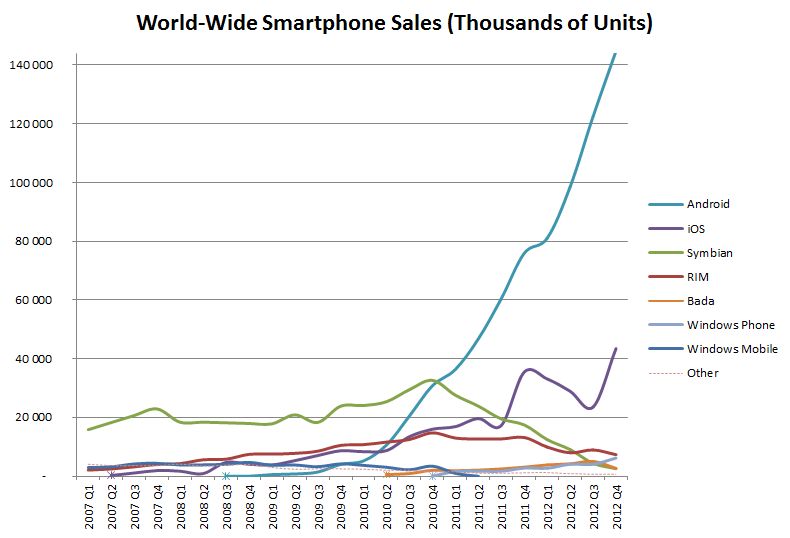
\includegraphics[width=0.8\columnwidth]{figs/World_Wide_Smartphone_Sales}
\caption{Worldwide Sales of various mobile OSs - from \citep{wikimobilesales} and \citep{gartnerq42012}}
\label{fig:mobilesales}
\end{center}
\end{figure}


\section{Android}
Started in 2003 by Andy Rubin and Android Inc. (previously the makers of the T-Mobile Sidekick), Android was acquired by Google Inc. in 2005\citep{businessweek2005}. ``Android was built from the ground-up to enable developers to create compelling mobile applications that take full advantage of all a handset has to offer. It was built to be truly open. For example, an application can call upon any of the phone's core functionality such as making calls, sending text messages, or using the camera, allowing developers to create richer and more cohesive experiences for users''\citep{ohaandroidoverview}. Since it's initial release in 2007\citep{oharelease2007}, Android has skyrocketed to the most used mobile OS in the world, with over 70\% marketshare, and 144 Million Android devices being sold in Q4 of 2012 alone\citep{gartnerq42012} - more than Apple had the entire year, as seen in Figure \ref{fig:mobilesales}.



\section{Goals of Mobile OSs}
For all these mobile OSs, they share many common goals and challenges. The diversity of hardware that smartphones were designed to replace, along other constraints and features, requires a mobile OS that's designed from the ground up to deal with many different challenges than the typical PC OS. Some of the main design challenges for a mobile OS are: 
\begin{smitemize}

\item Small memory footprint, battery conscious, and other resource constrictions

\item Access to a wide variety of personally identifiable information (PII)

\item Access a wide array of hardware

\end{smitemize}
In order to effectively enforce rules on battery consumption, low-latency UI, and personally identifiable information, a new security model was created, centered around the concept of the ``App''. 


%To understand the nature of modern mobile malware, we first examine the context. The two main models, that of iOS and Android, are compared and contrasted here.

\section{The ``App'' and Sandboxing}

In the mobile world, ``Apps'' are isolated and sandboxed programs, generally designed with one singular purpose. They lack dependencies, and generally are not as privileges as system software for performing many tasks. The mechanisms for accessing functionality outside of their sandbox is enforced by a set of policies the system holds, specific to that app. On some platforms, like iOS, only one app may run at any given time, and background computation is virtually non-existent (with some exceptions)\footnote{Minor amounts of computation can be done to compute background audio, and other isolated background tasks.}, along with many other restrictions. On Android and other platforms, many more features are available to apps, but in all cases, the ``app'' lifecycle is well defined and controlled by the system much more than on a PC OS.

There are various reasons for the tight sandboxing of mobile apps. Power and resource consumption are certainly a factor - mobile OSs generally reserve the right to kill apps if they attempt to allocate too much memory. Controlling access to hardware also helps in this: allowing apps to keep the phone awake could easily drain battery. However, another reason for sandboxing, and arguably more important, is protecting Personally Identifiable Information.

\subsection{Personally Identifiable Information}

Personally Identifiable Information (PII), as defined by the National Institute of Standards and Technology, is ``any information about an individual maintained by an agency, including (1) any information that can be used to distinguish or trace an individual‘s identity... and (2) any other information that is linked or linkable to an individual'' \citep{mccallister2010guide}. Mobile devices, having blended cameras, cell phones, GPS devices, and PCs into one device, have an extremely diverse amount of PII, from phone numbers, to contacts, to location history, to bank account numbers and pictures. For many of these datasets, mobile OSs actually organize them into databases with the intention of allowing 3rd parties access to them. Contact lists, SMS, Photographs and location history are available to apps on virtually every mobile platform in some official way. This is a driving motivation for a greatly improved security model for mobile OSs: controlling 3rd party software's access to PII. 

% Expand more on this.

\subsection{Digital Distribution Platform}

The final major difference between mobile OSs and PC OSs is the distribution of code. No mobile OS allows 3rd party code to be ran outside of the sandbox, and all of them require the user's consent before installing an app. All apps must be signed, and in general, there is 1 main distribution channel for all apps on a mobile OS. This tightly controlled distribution both aids in security, as well as controls the ecosystem around that mobile OS.

\subsection{Apple's App Store}
The first major digital distribution platform for mobile apps was Apple's App Store\citep{AppleAppStore}. Its model has been repeated by almost all major mobile app distribution platforms. The basic premise is simple: developers sign up to the app store, pay a fee (usually yearly), and submit fully-finished apps. A reviewer runs the app in a monitored sandbox, watches for unusual behavior, checks for stability and usability, and approves it. Once the app has been approved, it's released onto the app store, at which time anyone can download it. The approval process, as well as the high monetary fee, act as a way to ensure only safe and high-quality apps are available for that platform. In this type of platform, typically no apps may be installed from other sources. On iOS, initially this was the main method of security: if the app passed the inspection, it was acknowledged as safe and virtually unmonitored unless someone noticed something unusual and reported it. However, in recent years, after certain incidents (see section \ref{sec:path}), apps still must request permission from the user to perform certain tasks.

\subsection{Android Permissions}
Android's distribution platform takes a different approach, and at its core is also Android's security model: The Permission System (see section \ref{sec:permissions}). Android Apps declare when they are packaged what capabilities they will use, and the user reviews them at install time. If the user approves the app, it may use the requested capabilities whenever it wants: little restrictions are placed otherwise. With this barrier in mind, the Google Play Store (formerly known as the Android Market), or GPStore, opts for an alternate model to iOS, where the developer pays a smaller fee, and apps go through no formal approval process. After an app's submission, it's immediately released into the wild for users to download and run. The assumption Android uses is that the metadata the GPStore provides: App name, Developer Name, Description, Reviews and Ratings, are enough for the user to determine if the app should be trusted with the permission set it's given (see Figure \ref{fig:gpstoreapps}). In fact, Android even allows the device to accept apps from 3rd party sources, a practice known as ``sideloading'', although it's disabled by default. This has spawned a large number of 3rd party app sources, all of which rely on the Permission system for user protection.

%GPSTORE IMAGE AND CHART EXPLAINING THE LETTERS.

\begin{figure}[h]
\begin{center}
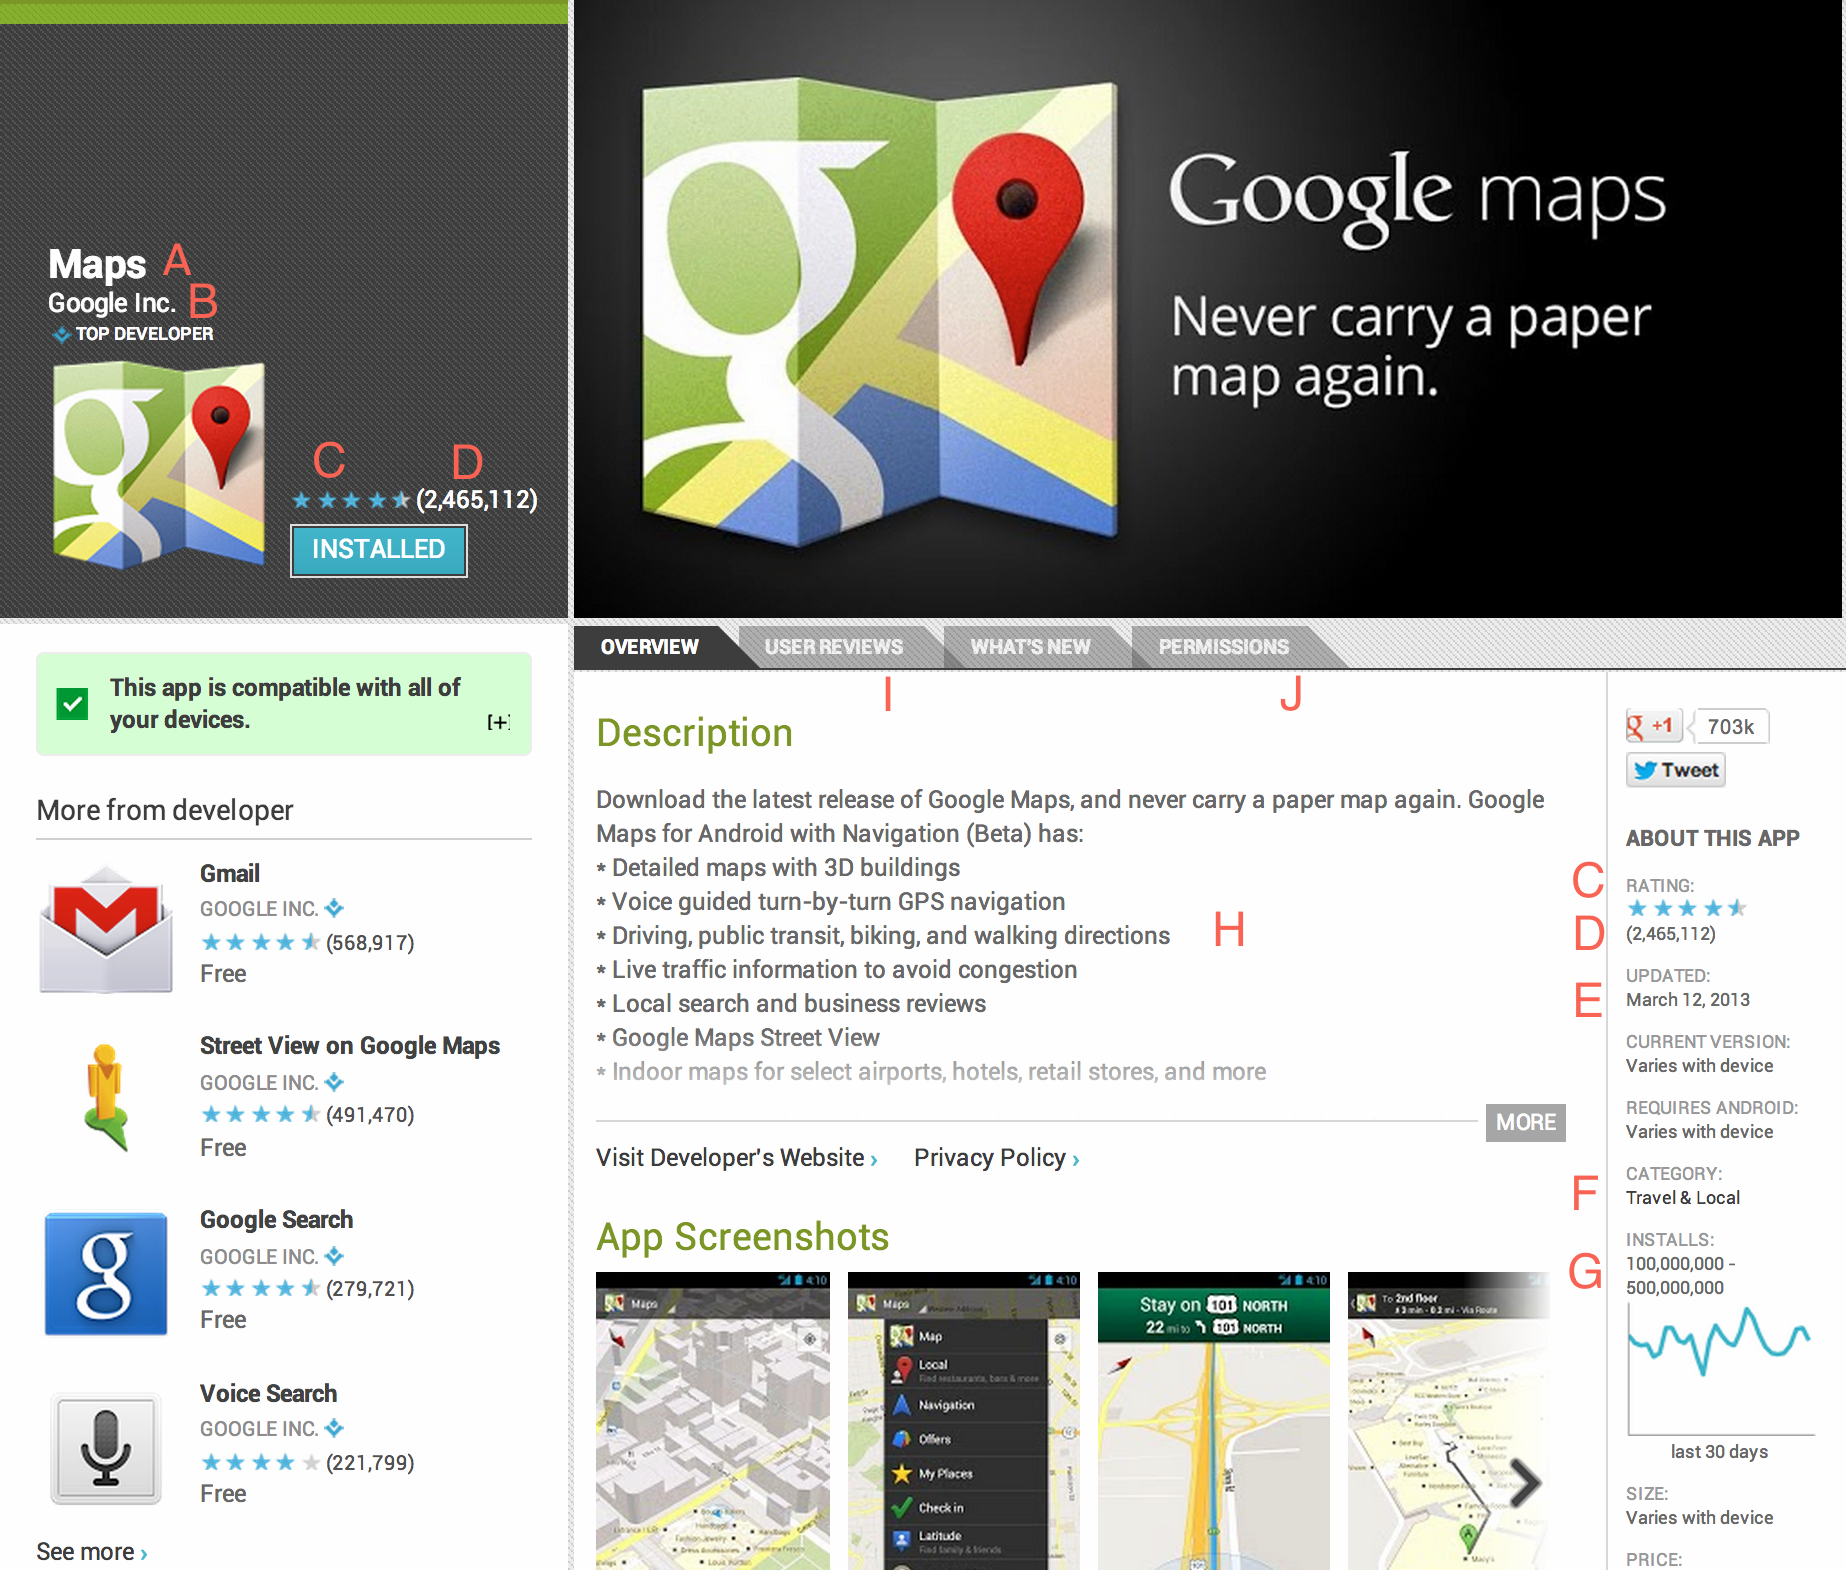
\includegraphics[width=0.9\columnwidth]{figs/GPStoreAppPage}
\caption{A sample page on the Google Play Store, see \ref{tab:gpstorekey}}
\label{fig:gpstoreapps}
\end{center}
\end{figure}

\begin{table*}[h]
\begin{small}
\begin{tabular}{l|l}

\textit{A} & App name  \\
\textit{B} & Developer Name  \\
\textit{C} & App Rating  \\
\textit{D} & Number of ratings  \\
\textit{E} & Date the app was last updated  \\
\textit{F} & Category in the Google Play Store it falls under  \\
\textit{G} & Number of installs (range, not exact number)  \\
\textit{H} & Description of the app  \\
\textit{I} & Reviews of the app  \\
\textit{J} & Permissions the app requests  \\

\end{tabular}
\end{small}
%\vspace{-0.2in}
\caption{Various properties of a Google Play Store app page}
\label{tab:gpstorekey}
%\vspace{-0.1in}
\end{table*}

%The core concept behind Android security - Permissions - are a static contract of capabilities. However, in this paper we propose an alternate means of conceptualizing security, which focuses on the interrelationship between the user's perception of the app, and the app's actual behavior. We call this the ``user-app agreement'', and will elaborate on it more later. 

\section{Mobile Malware}
Malware, as defined by the US Department of Homeland Security, is ``Short for malicious software. Programming (code, scripts, active content, and other software) designed to disrupt or deny operation, gather information that leads to loss of privacy or exploitation, gain unauthorized access to system resources, and other abusive behavior'' \citep{nash2005undirected}. Like PC OSs, malware is present on mobile OSs, although there are differences.


The tighter security model of Mobile OSs has a notable effect on mobile malware. With tight control in sandboxing, and app distribution, the usual viruses, trojans, and other exploits are more difficult to employ. The main vectors are either OS-level exploits, sneaking past the app review process, or through sideloading of apps. When looking at the two main mobile OSs, a stark contrast is shown. iOS has had  ``jailbreaking'' - privilege escalation exploits - dating back from its first release \citep{damopoulos2011isam}, whereas the first Android exploit was not discussed until 2010 by security researchers Papathanasiou and Percoco \citep{papathanasiou2010not}, and was not seen in the wild until early 2011\citep{castillo2010android}. On the contrary, no side-loading is possible for iOS, and there have been very few - if any - instances of malware sneaking past Apple's App Store review process, although it has happened\footnote{In July 2012, SecureList noticed an iOS app that uploaded all of the user's contacts to a remote location without their consent\citep{SecureList2012}, but others argued this was not as devious as made out to be\citep{trendmicroios2012} }. With 95\% of all mobile malware\citep{nq2013}, Android's malware situation is very much a product of the sideloading and lack of review process found in GPStore\citep{nq2013}. %Of all the mobile malware found for iOS and Android, over \temp{some percent} used no system-exploits at all, \temp{some percent} on the main app distribution platform.

 On mobile devices, one of the dominant goals of malware is to gather information that leads to loss of privacy, found in over 28\% of mobile malware in 2012 alone\citep{nq2013}. This trend, of malware that possesses no system exploits, but gathers information that leads to loss of privacy, known as Info Theft Malware, is one that Android's Permission-based security model is ill-equipped to handle. Android's permission system relies on the user to determine at install-time if a list of capabilities should be entrusted with the given app. The user is not given a say in how or when the capabilities may be used, nor the ability to reject specific capabilities. At the same time, the mechanisms that keep mobile OSs safe are forcing malware writers to use more subtle techniques, often times without exploits. This all works against the user.

In this paper, we attempt to address this key issue through various means. We first introduce several novel concepts for analyzing apps and malware on Android. We then analyze the state of Android apps and Permissions with the most comprehensive android app database available, Android Census. Finally, we propose several novel improvements to the Android security architecture, called AndroMEDA, aimed at building off of our conceptual work.

